%%%%%%%%%%%%%%%%%%%%%%%%%%%%%%%%%%%%%%%%%%%%%%%%%%%%%%%%%%%%%%%%%%%%%%%%%%%%%%%
%     STYLE POUR LES EXPOSÉS TECHNIQUES 
%         3e année INSA de Rennes
%
%             NE PAS MODIFIER
%%%%%%%%%%%%%%%%%%%%%%%%%%%%%%%%%%%%%%%%%%%%%%%%%%%%%%%%%%%%%%%%%%%%%%%%%%%%%%%

\documentclass[a4paper,11pt]{article}

\usepackage{exptech}       % Fichier (./exptech.sty) contenant les styles pour 
                           % l'expose technique (ne pas le modifier)

%\linespread{1,6}          % Pour une version destinée à un relecteur,
                           % décommenter cette commande (double interligne) 
                           
% UTILISEZ SPELL (correcteur orthographique) à accès simplifié depuis XEmacs
\usepackage{graphicx}
\usepackage{listings}
\usepackage{biblatex}
\addbibresource{rapport.bib}
\graphicspath{ {./images/} }

%%%%%%%%%%%%%%%%%%%%%%%%%%%%%%%%%%%%%%%%%%%%%%%%%%%%%%%%%%%%%%%%%%%%%%%%%%%%%%%

\title{ \textbf{Etude pratique \\
    Robot de combat darwinien} }
\markright{Robot de combat darwinien} 
                           % Pour avoir le titre de l'expose sur chaque page

\author{Daniel \textsc{Haus}, Etienne \textsc{Rebout}, \\
        Aurianne \textsc{Gilbert}, Antoine \textsc{Barroux} \\
        \\
        Tuteur : Christian \textsc{Raymond}}

\date{}                    % Ne pas modifier
 
%%%%%%%%%%%%%%%%%%%%%%%%%%%%%%%%%%%%%%%%%%%%%%%%%%%%%%%%%%%%%%%%%%%%%%%%%%%%%%%

\begin{document}          

\maketitle                 % Génère le titre
\thispagestyle{empty}      % Supprime le numéro de page sur la 1re page



\begin{abstract}
Notre projet consiste en la conception \cite{robocodeapi} et le développement d'un algorithme d'intelligence artificielle appliquée à un environnement de développement mis à disposition par IBM : Robocode. L'objectif est de faire apprendre à notre robot à se battre contre les robots par défaut fournis par Robocode à l'aide  d'un réseau de neurones dont les poids proviennent d'un apprentissage génétique. 
\end{abstract} 

\section{Remerciements}
Nous tenions à remercier notre tuteur Christian RAYMOND qui a été très disponible à la fois pour nous expliquer les concepts cachés derrière ce projet, et pour nous guider dans nos recherches et nos réflexions. Il a su nous donner les conseils nécessaires en terme d'implémentation afin que nous puissions avancer de manière efficace.\\
Nous souhaitions également remercier Pascal GARCIA qui s'est rendu disponible pour nous donner des pistes de réflexion autour du réseau de neurones et de son activation.

\section{Introduction}  

Ce projet s'inscrit dans le cadre des études pratiques proposées par l'INSA de Rennes, et a démarré en 2015 avec pour objectifs de réaliser une intelligence artificielle basée sur un réseau de neurones, le tout dans un environnement Robocode. Robocode est un jeu vidéo à but éducatif créé et distribué par IBM. Il nous permet de créer notre propre robot et de le faire se battre contre un ou plusieurs robots par défaut fournis par le jeu. Les robots sont représentés sous forme de tanks qui combattent dans un terrain. \\
Une partie de Robocode commence par la création d'un robot qui est envoyé en combat contre un adversaire. C'est un combat dans lequel il va devoir récupérer des informations et les utiliser dans son perceptron afin de prendre des décisions. Notre robot est constitué d'un radar afin d'apercevoir l'ennemi, d'un canon afin de tirer sur son adversaire et de chenilles pour se diriger. Ces trois composants peuvent tourner indépendamment les unes des autres. 

\subsection{Outils utilisés}

\subsection{Robocode}
L'environnement du jeu dans lequel sont simulés tous les combats entre les robots.

\subsubsection{Java}
Robocode propose deux langages pour le développement de l'intelligence artificielle des robots : le Java ou le .NET. Darwini existant depuis maintenant trois ans, nous avons utilisé le Java car c'est le langage qui a été utilisé depuis le début du projet.

\subsubsection{XML}
Chaque robot généré est stocké sous la forme de son perceptron, au format XML. 

\subsubsection{IntelliJ}
L'IDE IntelliJ était utilisé par le groupe précédent et nous avait été présenté en cours. De plus il nous semblait plus simple d'utilisation qu'Eclipse, c'est pourquoi nous l'avons choisi.

\subsubsection{GitHub}
Nous avons créé un répertoire GitHub afin de pouvoir travailler autant chez nous qu'à l'INSA. De plus Git gère le fait que plusieurs personnes travaillent simultanément sur le même fichier ou permet de dupliquer le projet en "branche" lorsqu'une modification importante est en cours mais qu'elle ne fonctionne pas encore ce qui permet à la fois d'avoir un prototype fonctionnel et un prototype en développement. Nous avons choisi GitHub contrairement à GitLab car nous voulions conserver ce projet open-source.

\subsubsection{API de Robocode}
La documentation de Robocode fournie par IBM est à la base de ce projet. Elle contient à la fois une documentation complète du fonctionnement du jeu, mais également la documentation technique nous permettant de récupérer les données du jeu pendant un combat, sans quoi ce projet ne pourrait avancer.

\section{Analyse de l'existant}  

Comme expliqué plus haut, ce projet existe depuis 3 ans et consiste donc en une reprise et évolution d'un code existant. 

\subsection{La conception}

Ce serait pas mal de mettre l'uml ici ou d'expliquer un peu leur ancien modèle de données (= pas prore, en fouillis, les méthodes étaient situées random)

Petite figure de l'ancien UML serait top



Pour inclure une image, on doit aussi la convertir en EPS, avec
la commande \texttt{convert}\footnote{
disponible aussi sous Unix/Linux et à privilégier 
car elle génère un EPS tout à fait standard 
(au contraire de nombreux pilotes Windows).}
\texttt{~image image.eps}, qui accepte pratiquement tous les formats d'images.


\subsection{L'application}

D'un point de vue de l'application, de nombreuses fonctionnalités étaient déjà en place. Voici celles sur lesquelles nous nous sommes basé : 

\begin{itemize}
\item Lancement d'un combat entre notre robot et un robot par défaut fourni par Robocode.
\item Récupération des données pendant et après le combat.
\item Gestion du perceptron à l'aide d'une classe Matrix.
\item Gestion des données d'entrée et de sortie du perceptron.
\item Apprentissage des poids du perceptron par un algorithme génétique.
\end{itemize}

\subsection{Conclusion} 
 
Après l'analyse de l'existant, on pourrait croire que le projet touchait déjà à sa fin au moment où nous l'avons repris et pourtant, nous avons apporté beaucoup de modifications dans l'implémentation du processus à cause de problèmes majeurs, comme par exemple le système d'apprentissage génétique qui n'était pas fonctionnel. Nous verrons plus en détail dans la section suivante les problèmes d'implémentation rencontrés et les décisions que nous avons prises par rapport à ceux-ci.



\section{Travail effectué}

\subsection{Conception et modélisation des données}
Nous avons décidé de revoir le modèle des données qui était en place afin de faciliter la compréhension du code. Nous avons donc décidé de nous baser sur 4 classes principales : 

\begin{itemize}
    \item NaturalSelection : elle correspond au point d'entrée de l'application, c'est elle qui lance l'algorithme génétique et qui fixe les paramètres de celui-ci.
    \item Population : elle regroupe toutes les méthodes concernant la gestion des individus, la création de la génération suivante à partir de la génération courante.
    \item Individual : elle permet de gérer chaque individu de la population, et elle regroupe notamment les méthodes permettant de simuler les combats dans robocode et donc de calculer la fitness.
    \item NeuralNetwork : elle correspond au perceptron de chaque individu et permet de conserver les poids utilisés dans le réseau de neurones par chaque individu.
\end{itemize}





\subsection{Modélisation du perceptron}

\subsubsection{Les données d'entrées}

\paragraph{Rôle}
Les données récupérées par le robot sont essentielles à la prise de décisions car elles représentent les neurones d'entrée du perceptron. Le robot récupère des informations importantes pour le jeu telles que la position de l'ennemi, sa direction ou encore ses points de vie restant. La difficulté consiste à trier ces informations et ne garder que les plus pertinentes. En outre, il a fallu traiter certaines données afin d'optimiser le comportement de notre robot. C'est le cas pour la position de l'ennemi, que nous pouvons récupérer grâce à l'API, qui se révèle bien plus efficace si on lui donne directement la distance qui sépare notre robot de son adversaire. Le fonctionnement est le même pour la distance séparant notre robot du prochain mur, afin qu'il se déplace correctement.

\paragraph{Données choisies}
Les données que nous avons choisi de garder sont les suivantes :

\begin{itemize}
\item L'angle entre la direction de notre robot et la position du robot adverse.
\item L'angle entre la direction du canon de notre robot et la position du robot adverse.
\item L'angle entre la position du radar de notre robot et la position du robot adverse.
\item La distance entre notre robot et l'adversaire.
\item L'énérgie restante de notre robot.
\item La vitesse de notre robot.
\item La vitesse de l'adversaire.
\item La distance entre notre robot et le mur le plus proche.
\end{itemize}

\subsubsection{Les données de sortie}

\paragraph{Rôle}
Les données de sortie représentent les décisions que le robot va prendre après traitement par le perceptron. Pour permettre à notre robot d'apprendre plus facilement, on ne lui apprend que quelques comportements à la fois, voire un seul. Par exemple, nous avons privilégié le déplacement du robot (ne pas entrer en collision avec les murs, éviter les balles de l'adversaires, etc) à la décision de tirer. En effet, le cas écheant, notre robot restait immobile et tirait sur l'adversaire en continu, sans adopter de réelle stratégie. Sachant que dans l'environnement Robocode, le robot qui tire sur son adversaire perd de la vie à chaque tir, cette conduite était suicidaire.

\paragraph{Données choisies}
Les données de sortie retenues sont :

\begin{itemize}
\item Décision de tirer.
\item Décision de tourner.
\item Décision de tourner le radar.
\item Décision de tourner le canon.
\item Décision d'avancer.
\end{itemize}

\subsubsection{Perceptron}
Le perceptron correspond à l'ensemble des liaisons et des opérations constituant le réseau de neurones et permettant de lier les données d'entrée aux données de sortie. 

Un perceptron multicouche est un classiffieur dit neuronal formel organisé en
plusieurs couches au sein desquelles une information circule des couches d'entrée
vers les couches de sortie. Ce modèle s'inspire du fonctionnement de nos neurones.
Dans notre cas nous utilisons trois couches différentes :

\begin{itemize}
\item la couche d'entrée qui récupère nos données d'entrée
\item la couche de neurones cachés
\item la couche de sortie qui nous permet de prendre des décisions
\end{itemize}

Dans un perceptron, tous les neurones de chaque couche sont connectés à tous les
neurones de la couche suivante. Ainsi, tous les neurones d'entrée sont connectés
aux neurones de la couche cachée. De même, les neurones de la couche cachée sont
connectés aux neurones de sortie. L'important dans un perceptron est que chacune
de ces connexions entre neurones est caractérisée par un coefficient de pondération,
qui représentent les poids du perceptron. 

\begin{figure}[!h]
\centering
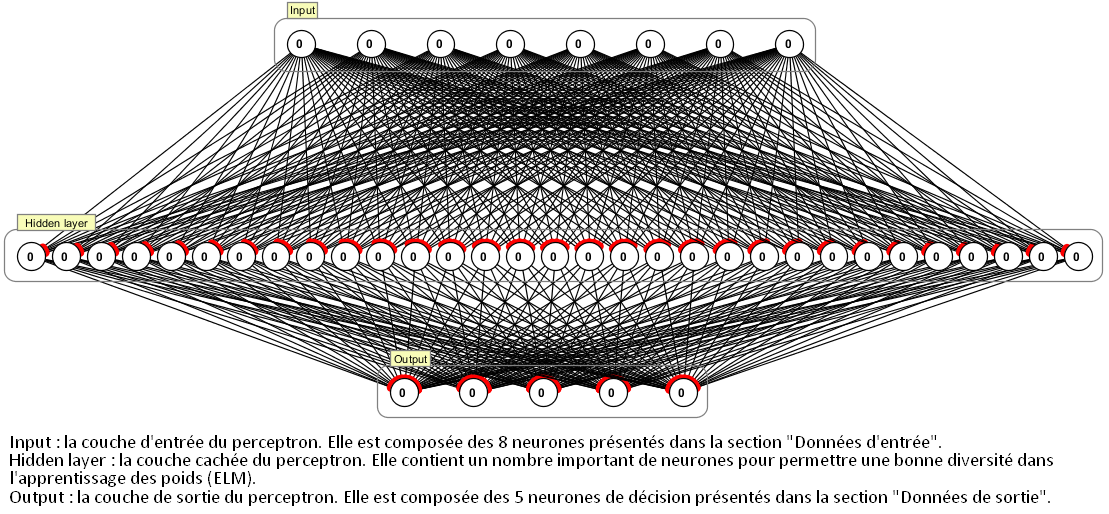
\includegraphics{images/global_network.png}
\caption{Représentation du perceptron de Darwini}
\label{darwini_perceptron}
\end{figure}

\subsubsection{Fonctionnement}
Le perceptron fonctionne de la manière suivante :
Chaque donnée d'entrée est représentée par un neurone dans la couche d'entrée.
Chaque neurone de la couche cachée prend pour valeur la somme des produits des
valeurs des neurones d'entrée multipliée par la valeur des poids attribués à chaque
connexion.
Chaque neurone de la couche de sortie correspond à une action du robot. Il est le
résultat de la multiplication des valeurs des neurones de la couche cachée, auxquelles
nous avons appliqué une fonction Relu, par les poids des liens entres neurones cachés
et neurones de sortie.
Ensuite, notre robot prend sa décision en fonction de la valeur du neurone de sortie correspondant.

\subsubsection{Implémentation}
Le perception est implémenté en 4 classes Java.
\begin{itemize}
\item Une classe InputData qui récupère les données fournies par le jeu. Les neurones d'entrées sont donc les valeurs numériques fournies par le jeu.
\item Une classe OutputData qui définit les neurones de sortie donc les décisions du robot. Par exemple le neurone qui correspond au tir peut contenir la valeur 1 ce qui signifie que le robot doit tirer ou la valeur 0 pour ne pas tirer.
\item Une classe NeuralNetwork implémentant le perceptron. Un perceptron est représenté comme l'association de deux matrices, l'une représentant les poids des liens des couches
entrée-cachée et l'autre les poids des liens des couches cachée-sortie. Ces poids sont générés de manière aléatoire.
Ainsi nous disposons d'une fonction qui prend les valeurs des données d'entrée
choisies et les transforme en un vecteur et effectue les différentes applications
numériques. On obtient donc une matrice dont on prendra autant de premiers coefficients qu'il y a de neurones de sortie.
\item Une classe Matrix car les poids des différents neurones sont présentés sous forme matricielle.
\end{itemize}



\subsection{Apprentissage génétique}

Pour obtenir un robot performant, il faut donc que les poids du perceptrons soient adaptés. L'intérêt de l'algorithme génétique est que le robot va trouver lui-même la combinaison idéale des poids de son perceptron. Pour ce faire, nous allons utiliser la théorie de l'évolution.

\subsubsection{La Fitness}
Pour commencer il nous faut savoir évaluer la performance d'un robot lors d'un combat. Pour cela, nous utilisons une méthode fitness qui, à la fin de chaque combat, nous génère un résultat qui sera le score du robot. Cette fitness peut être changée en fonction des résultats que l'on souhaite obtenir. Par exemple, si l'on souhaite que notre robot favorise le comportement "éviter les murs", on peut enlever des points au robot à chaque fois qu'il entre en collision avec un mur. Ainsi, lorsque l'algorithme génétique va sélectionner les meilleurs individus, ce sont les individus les mieux adapté au comportement "éviter les murs" qui seront conservé, et leur gène sera retransmis aux générations futures. La fitness telle qu'elle était présente au départ était basée sur les dégâts que l'on cause à l'adversaire, le fait de gagner une partie et le taux de tirs réussis. Nous avons décider d'adopter une autre méthode car nous pensons qu'il est presque impossible de faire prendre les décisions basique à notre robot en se basant uniquement sur leur taux de victoire. En effet, il est très dur avec cette fitness de séparer les robots les plus mauvais des robots "un peu moins mauvais", car ils perdaient tous leur combat en tirant aléatoirement.
Nous avons utilisé beaucoup de fitness différentes pour essayer de faire adopter des comportements différents à notre robot. Voici la fitness que nous avons testé pour le comportement "éviter un mur" : 

\begin{lstlisting}
fitness = 20 * bulletDamage
                            + 10 * survival
                            + ramDamage
                            + 5*totalScore
                            + victory
                            - 1000*hitsWall
                            - 5*hitByBullet
 \end{lstlisting}
 Elle est donc influencée très négativement si jamais le robot entre en collision avec un mur.

\subsubsection{Populations et individus}
La première étape de l'algorithme génétique consiste en la création d'une population d'individus. Chacun de ces individus va combattre un robot prédéfini de Robocode, combat grâce auquel on va pouvoir calculer sa fitness. Les individus sont alors classés du meilleur au plus mauvais. La population suivante sera générée à partir des meilleurs individus de cette génération. Chaque nouvel individu aura un perceptron dont les poids seront calculés à partir de l'écart-type et de la moyenne des poids des meilleurs individus de la génération précédente. Nous incluons également dans la nouvelle génération un certain nombre des meilleurs individus de la génération précédente. Le but de cet algorithme est d'obtenir l'individu le mieux adapté aux contraintes imposées par la fitness après un grand nombre de générations.

\subsubsection{Refonte de l'algorithme génétique}
Nous avons décidé de reprendre entièrement l'algorithme génétique qui posait des problèmes d'implémentation. La parallélisation du calcul de la fitness a été supprimée car elle causait des problèmes de données manquantes. Nous avons également modifié la façon de générer les individus en réalisant un tirage aléatoire gaussien à partir de la moyenne et de l'écart-type des poids de la génération précédente. Cette implémentation permet de faire converger les individus vers une valeur optimale sans conserver obligatoirement le poids de l'un de ses deux parents. Dans la première implémentation, tous les individus étaient identiques car tous les individus étaient générés à partir des deux mêmes meilleurs individus de la génération. 
Nous avons également réimplémenté le système de mutation qui permet d'apporter de la diversité génétique à nos individus. Ces mutations vont apparaître pour environ un poids sur dix et consiste à faire varier le poids de départ entre -10\% et +10\%.


\section{Expérimentations et tests}
Après quelques tests, nous avons conclu qu'il serait particulièrement difficile de faire apprendre tous les comportements à adopter en combat à notre robot. En effet, il y a beaucoup de facteurs à prendre en compte, c'est pourquoi nous avons décidé de faire des tests sur un comportement à la fois. Voici les différents comportements que nous avons ciblé lors de nos tests.

\subsection{Se déplacer sans rentrer dans les murs}
Le déplacement est un point central du combat dans Robocode. L'objectif est de faire en sorte que le robot se déplace tout au long du combat dans le but d'esquiver un maximum de tirs ennemis. La base du déplacement est d'éviter les murs, c'est pourquoi nous avons utilisé une fonction de fitness qui punit sévèrement les collisions avec les murs. Nous avons restreint la liste des données d'entrée et de sortie comme présenté dans la figure ci-dessous. 

\begin{figure}[!h]
\centering
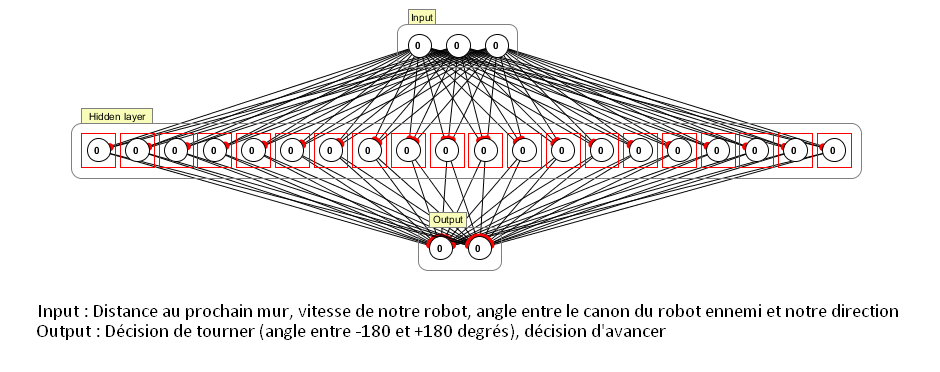
\includegraphics{images/move_network.png}
\caption{Perceptron utilisé pour se déplacer et éviter les murs}
\label{move_perceptron}
\end{figure}

Le problème majeur que nous avons rencontré est que le robot n'était pas contraint de se déplacer car nous n'avons pas réussi à récupérer la distance parcourue par notre robot pendant le combat. Cette donnée nous aurait permis de favoriser un gros déplacement dans notre fonction de fitness et donc favoriser les individus qui se déplacent beaucoup. Au lieu de cela, le robot préfère rester figé étant donné qu'il n'entre pas en collision avec les murs et obtient donc un score de fitness correct. La solution idéale aurait été de fragmenter le terrain de combat en une grille, nous permettant ainsi de favoriser les individus ayant visité le plus de cases de la grille et donc ceux qui ont réussi à se déplacer le plus dans le terrain de combat.


\subsection{Orienter son radar pour suivre l'ennemi}
L'orientation du radar est un comportement légèrement différent des autres étant donné que l'on est capable de savoir comment agir au mieux pour toujours voir l'ennemi. En effet, le radar nous permet, s'il est orienté vers le robot ennemi, d'accéder aux informations de l'adversaire et donc de connaître les données de base nous permettant de faire tourner le réseau de neurones. Nous avons commencé par implémenter en "dur" ce comportement, basé sur l'angle entre la direction de notre radar et la direction du robot ennemi. Le fait de fixer ce comportement nous a permi notamment de faire nos tests sur les autres comportements et surtout celui concernant le tir. \\
Cependant, nous avons tout de même essayé de faire apprendre ce comportement au robot, une fois encore en restreignant les données fournies au perceptron.

\begin{figure}[!h]
\centering
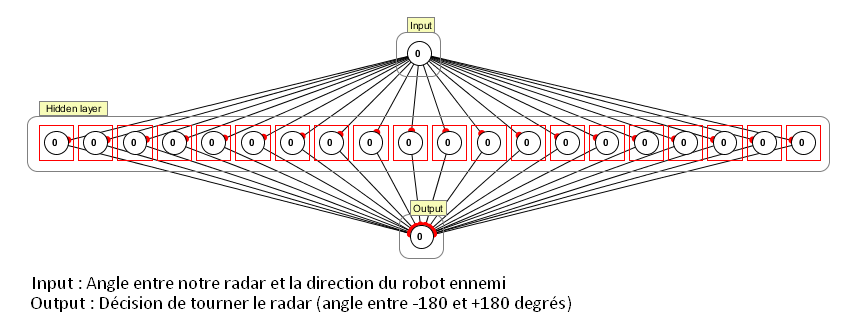
\includegraphics{images/radar_network.png}
\caption{Perceptron utilisé pour suivre l'ennemi avec notre radar}
\label{radar_perceptron}
\end{figure}

Nous avons utilisé une fonction de fitness qui calcule le ratio entre le temps passé dans le jeu en voyant l'ennemi et le temps total du combat. Le problème majeur vient du fait qu'au départ, on ne voit pas le robot ennemi étant donné que le radar n'est pas ciblé sur l'adversaire au début du combat. De ce fait, le réseau de neurones ne peut pas être utilisé puisqu'il faut voir l'adversaire pour en extraire les informations nécessaires.


\subsection{Orienter son canon pour tirer}
Dernier point fondamental d'un combat Robocode : viser et tirer sur l'ennemi. Ce comportement est assez stratégique puisque chaque tir enlève de l'énergie à notre robot, c'est donc un point à prendre en compte dans nos données fournies au perceptron. La décision de tirer est différente des autres puisqu'il s'agit vraiment d'une action binaire : tirer ou non. Il faut donc faire un compromis entre tirer sans arrêt et ne toucher que très rarement, ou tirer seulement quand on est certain de toucher.


\begin{figure}[!h]
\centering
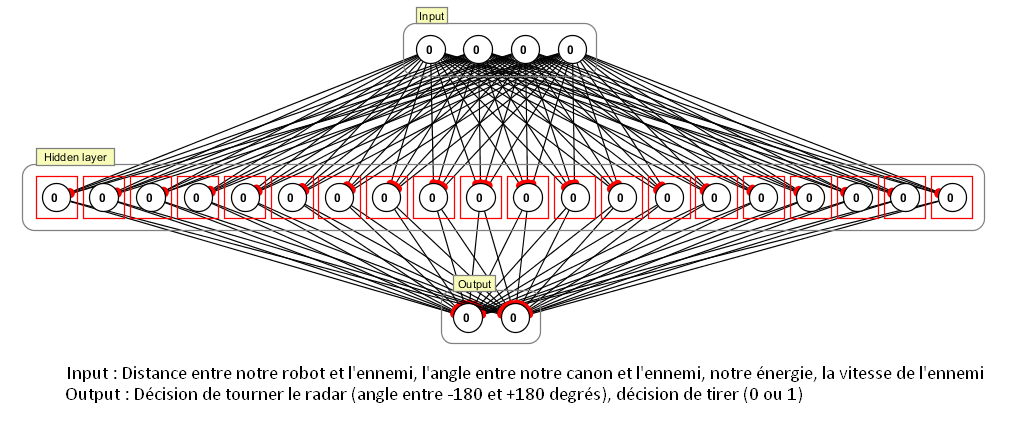
\includegraphics{images/tir_network.png}
\caption{Perceptron utilisé pour bouger le canon et tirer}
\label{canon_perceptron}
\end{figure}


\newpage


\printbibliography
\end{document}

%%%%%%%%%%%%%%%%%%%%%%%%%%%%%%%%%%%%%%%%%%%%%%%%%%%%%%%%%%%%%%%%%%%%%%%%%%%%%%%
